\documentclass{beamer}

\usepackage{enumitem}
\usepackage{amsmath,amssymb}
\usepackage{tikz}
\usepackage{graphicx}
\usepackage{multicol}
\usepackage[per-mode=fraction]{siunitx}

\usetheme{Boadilla}
\usecolortheme{orchid}

\usetikzlibrary{calc}

\tikzset{>=stealth}


\title{PHYS2350: Forces}
\author{Dr. Wolf}
\date{Fall 2024}

\begin{document}

\begin{frame}
  \titlepage
\end{frame}

\begin{frame}
  {Part \textrm{I}(a): Free-body diagrams}
  \begin{columns}
    \begin{column}{0.5\textwidth}
      (i)
      \begin{center}
        \begin{tikzpicture}
          \fill[white] (-1.5,-1.5) rectangle (1.5,1.5);
          \draw[->] (0,0) -- (0,-1) node [right] {$F^{(G)}$};
          \fill (0,0) circle (0.1);
        \end{tikzpicture}
      \end{center}
      \[
        \vec{a} = (0,-g)
      \]
    \end{column}
    \begin{column}{0.5\textwidth}
      (ii)
      \begin{center}
        \begin{tikzpicture}
          \fill[white] (-1.5,-1.5) rectangle (1.5,1.5);
          \draw[->] (0,0) -- (0,-1) node [right] {$F^{(G)}$};
          \draw[->] (0,0) -- (0,1) node [left] {$F^{(\text{Drag})}$};
          \fill (0,0) circle (0.1);
        \end{tikzpicture}
      \end{center}
      \[
        \vec{a} = (0,0)
      \]
    \end{column}
  \end{columns}
\end{frame}

\begin{frame}
  {Part \textrm{I}(b) Graph}
  Your graphs should look something like this:
  \begin{center}
    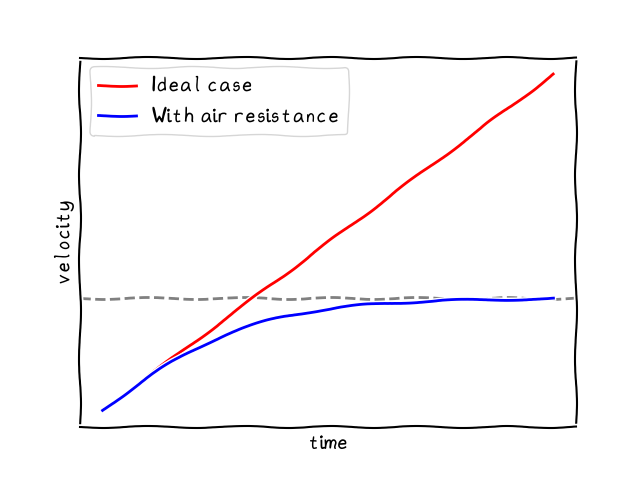
\includegraphics[width=0.7\textwidth]{velTimePlot.png}
  \end{center}
\end{frame}

\begin{frame}
  {Part \textrm{I}(c): Free-body diagrams}
  \begin{columns}
    \begin{column}{0.5\textwidth}
      (i)
      \begin{center}
        \begin{tikzpicture}
          \fill[white] (-1.5,-1.5) rectangle (1.5,1.5);
          \draw[->] (0,0) -- (0,0.5) node [left] {$F^{(\text{Drag})}$};
          \draw[->] (0,0) -- (0,-1) node [right] {$F^{(G)}$};
          \fill (0,0) circle (0.1);
        \end{tikzpicture}
      \end{center}
      Acceleration is \textit{down}:
      \[
        \left|\vec{a}\right| < g
      \]
    \end{column}
    \begin{column}{0.5\textwidth}
      (ii)
      \begin{center}
        \begin{tikzpicture}
          \fill[white] (-1.5,-1.5) rectangle (1.5,1.5);
          \draw[->] (0.05,0) -- +(0,-1) node [right] {$F^{(G)}$};
          \draw[->] (-0.05,0) -- +(0,-0.5) node [left] {$F^{(\text{Drag})}$};
          \fill (0,0) circle (0.1);
        \end{tikzpicture}
      \end{center}
      Acceleration is \textit{down}
      \[
        \left|\vec{a}\right| > g
      \]
    \end{column}
  \end{columns}
  \begin{block}
    The drag force has the same \textit{magnitude} at both instants, but a different \textit{direction}
  \end{block}
\end{frame}

\begin{frame}
  {Part \textrm{II} - Calculating terminal speed}
  Assuming vertically downward is the positive direction
  \begin{enumerate}[label=(\alph*)]
    \item $v>0$ implies:
    \[ ma = mg - c_1 v - c_2 v^2 \]
    \item $v<0$ implies:
    \[ ma = mg + c_1 v + c_2 v^2 \]
    \item For terminal velocity, $a=0$. This implies:
    \[
      0 = mg - c_2 v_T^2 \implies v_T = \sqrt{\frac{mg}{c_2}}
    \]
  \end{enumerate}
  \begin{exampleblock}
    {Checking units}
    Since $c_2 v^2$ is a force, $c_2$ must have units of:
    \[
      \frac{\text{Force}}{(\text{velocity})^2} =
      \frac{\si{\newton}}{\si{\meter^2\per\second^2}}
      = \frac{\si{\kilo\gram\meter\per\second^2}}{\si{\meter^2\per\second^2}} = \si{\kilo\gram\per\meter}
    \]
  \end{exampleblock}
\end{frame}


\end{document}